\documentclass[11pt]{article}
\setlength{\oddsidemargin}{0in}
\setlength{\evensidemargin}{0in}
\setlength{\textwidth}{6.5in}
\setlength{\parindent}{0in}
\setlength{\parskip}{\baselineskip}

\usepackage{amsmath,amsfonts,amssymb}
\usepackage{fancybox}
\usepackage{subfiles}
\usepackage{enumitem, tabularx, booktabs, ragged2e}
\usepackage[margin=1in]{geometry}
\usepackage{listings, lstautogobble}
\usepackage{alltt}
\usepackage{tikz}
\usepackage{tabularx}
\usepackage{graphicx}
\usepackage{xcolor}
\usepackage{blkarray}
\usepackage[bottom]{footmisc}
\usepackage{rotating}
\usepackage{wasysym}
\usepackage{rotating}
\usepackage[hidelinks]{hyperref}
\graphicspath{{images/}{./img/}}
\usepackage{verbatimbox}
\usepackage{tablefootnote}
\newcolumntype{L}{>{\centering\arraybackslash}m{1cm}}

% colors in math environment
\usepackage{xcolor}
\definecolor{orange}{rgb}{1,0.5,0}
\definecolor{blue}{rgb}{0.22, 0.58, 0.82}
\definecolor{green}{rgb}{0.2, 0.65, 0.32}
\definecolor{red}{rgb}{0.91, 0.26, 0.2}
\definecolor{purple}{rgb}{0.46, 0.21, 0.68}
\makeatletter
\def\mathcolor#1#{\@mathcolor{#1}}
\def\@mathcolor#1#2#3{%
	\protect\leavevmode
	\begingroup
	\color#1{#2}#3%
	\endgroup
}
\makeatother

\allowdisplaybreaks

% Label subfigures as 1(a) instead of 1a
\usepackage[labelformat=simple]{subcaption}
\renewcommand\thesubfigure{(\alph{subfigure})}
\usetikzlibrary{automata,positioning}

% Var, MSE, Bias
\newcommand{\Var}{\text{Var}}
\newcommand{\var}{\text{var}}
\newcommand{\Cov}{\text{Cov}}
\newcommand{\cov}{\text{cov}}
\newcommand{\corr}{\text{corr}}
\newcommand{\MSE}{\text{MSE}}
\newcommand{\bias}{\text{Bias}}
\newcommand{\E}{\mathbb{E}}
\newcommand{\iid}{\stackrel{\text{i.i.d.}}{\sim}}

% Norm and absolute value
\newcommand{\norm}[1]{\left\lVert#1\right\rVert}
\newcommand{\abs}[1]{\left\lvert#1\right\rvert}


\newcommand{\g}[1][G]{\mathcal{#1}}

% argmax and argmin
\DeclareMathOperator*{\argmin}{argmin} % no space, limits underneath in displays
\DeclareMathOperator*{\argmax}{argmax} % no space, limits underneath in displays

% Decorators
\newcommand{\dinkus}{\begin{center}***\end{center}}

% Make code look nicer
\definecolor{codegreen}{rgb}{0,0.6,0}
\definecolor{codegray}{rgb}{0.5,0.5,0.5}
\definecolor{codepurple}{rgb}{0.58,0,0.82}
\definecolor{backcolour}{rgb}{0.95,0.95,0.92}
\lstdefinestyle{mystyle}{
    backgroundcolor=\color{backcolour},   
    commentstyle=\color{codegreen},
    keywordstyle=\color{magenta},
    numberstyle=\tiny\color{codegray},
    stringstyle=\color{codepurple},
    basicstyle=\ttfamily\footnotesize,
    breakatwhitespace=false,         
    breaklines=true,                 
    captionpos=b,                    
    keepspaces=true,                 
    numbers=left,                    
    numbersep=5pt,                  
    showspaces=false,                
    showstringspaces=false,
    showtabs=false,                  
    tabsize=2
}
\lstset{style=mystyle}

\begin{document}

\begin{center}
  \setlength\fboxsep{0.5cm}
  \fbox{\parbox{\textwidth}{
  \textbf{STAT 517: Stochastic Modeling II} \hfill \textbf{Winter 2023}
 \begin{center}
	 {\Large\textbf{Lab 3 Notes}} \\
	 February, 23 2023 \\
 \end{center}
	\textit{Instructor: Abel Rodriguez} \hfill \textit{TA: Apara Venkat}
	}}
\end{center}

\textit{These notes are meant to accompany the discussions in the lab. They contain derivations for mathematical quantities estimated in the lab and other miscellaneous information. They have not been proofread and may contain typos. Please email aparav@uw.edu if you catch errors.}

\begin{enumerate}

\item
\begin{enumerate}
\item Say that we are observing a homogeneous Poisson process for a total time $T$. And we have arrival times $\{t_1, t_2, \dots, t_n\}$ generated with rate $\lambda$. We know that $t_i - t_{i-1}$ comes from an Exponential distribution with rate $\lambda$. Suppose we define $t_0 = 0$. Then, the likelihood is
\begin{align*}
	\mathcal{L}(\lambda) &= \prod_{i=1}^n \lambda e^{-\lambda (t_i - t_{i-1})} \\
	&= \lambda^n e^{-\lambda t_n} \\
	\implies \ell(\lambda) &= \log \mathcal{L}(\lambda) \\
	&= n \log \lambda - \lambda t_n
\end{align*}
Setting the score equation to zero gives us $\widehat{\lambda} = n / t_n$. We can also find the asymptotic variance by,
\begin{align*}
	\Var(\widehat{\lambda}) &= \left( - \E \frac{\partial^2 \ell}{\partial \lambda^2} \right)^{-1} \\
	&= \left( \E \left[ N(T) / \lambda^2 \right] \right)^{-1}
\end{align*}
where $N(T)$ is the number of events we observe in time $T$. Thus, $\E N(T) = \lambda T$. And,
\begin{align*}
	\Var(\widehat{\lambda}) &= \frac{\lambda}{T} \\
	\implies \widehat{\Var}(\widehat{\lambda}) &= \frac{\widehat{\lambda}}{T}
\end{align*}

\item If we assume that the first observation is censored, we know the first event occurs at some time $t \geq t_1$. Similarly, we know that the event after $t_n$ occurs at some time $t \geq T - t_n$. Combining these into the likelihood, we have
\begin{align*}
	\mathcal{L}(\lambda) &= P(\text{event 1 occurs after } t_1) P(\text{event } n + 1 \text{ occurs after } T - t_n) \prod_{i=2}^n \lambda e^{-\lambda (t_i - t_{i-1})} \\
	&= e^{-\lambda t_1} e^{-\lambda (T - t_n)} \lambda^{n-1} e^{-\lambda (t_n - t_1)} \\
	&= \lambda^{n-1} e^{-\lambda T}
\end{align*}
Similar to part (a), we can calculate the MLE and its variance as
\begin{align*}
	\widehat{\lambda} &= \frac{T}{n - 1} \\
	\Var(\widehat{\lambda}) &= \frac{\lambda^2}{\lambda T - 1} \\
	\implies \widehat{\Var}(\widehat{\lambda}) &= \frac{\widehat{\lambda}^2}{\widehat{\lambda} T - 1}
\end{align*}
Notice that for large enough $T$ (and therefore $n$), this behaves similar to the estimator in part (a).

\item We know that the arrival times, conditioned on the number of events, come from a uniform distribution on $[0, T]$. We can use this fact to perform the Kolmogorov-Smirnov (KS) test. The KS test essentially compares the empirical CDF, $F_n$, with a theoretical CDF $F$. The test statistic is,
\begin{align*}
	D_n &= \sup_x \abs{F_n(x) - F(x)}
\end{align*}

Glivenko-Cantelli theorem says that $D_n \stackrel{a.s.}{\to} 0$ where a.s. is almost sure convergence. In fact, Donsker's theorem gives us a convergence rate $\sqrt{n} D_n = O_P(1)$. Under the null hypothesis, $\sqrt{n} D_n \stackrel{d}{\to} \sup_{t \in [0,T]} \abs{X(F(t))}$ where $X(t)$ is a Brownian bridge process i.e., it is a mean-zero Gaussian process with the covariance function $(h_1, h_2) \to E (h_1 h_2) - \E h_1 \cdot \E h_2$. This is also called the Kolmogorov distribution.\footnote{The results in this paragraph should be familiar if you have taken a course in advanced probability or advanced statistical theory equivalent to the STAT 580 sequence. However, this is not a prerequisite to performing a KS test.}

Theoretical details aside, we can use this test-statistic to perform the KS test. We just need to provide a null distribution. In our case, it is $\text{Unif}[0, T]$. Generally, the KS test needs a lot of data to reject the null. And sometimes Q-Q plots can serve as a better method to assess goodness-of-fit.

\end{enumerate}

\hfill $\blacksquare$


\clearpage
\item
\begin{enumerate}
\item Consider a region $S$. Observations are recorded on this region at locations $\{s_i\}_{i=1}^n$ where $s_i = (x_i, y_i) \in S$. We want to model these observations as a non-homogeneous Poisson point process (NHPPP). The distribution of the number of points in a region $A \subseteq S$ is then,
\begin{align*}
	N(A) &\sim \text{Poisson}(\Lambda(A)), \\
	\Lambda(A) &= \int_A \lambda(s) ds
\end{align*}
where $\lambda$ is called the intensity function. We can associate $\lambda$ to a density $f$ as
\begin{align*}
	f(s) &= \frac{\lambda(s)}{\Lambda(S)}
\end{align*}
Further, if $A \cap B = \phi$ for two sets $A, B \subseteq S$, then $N(A) \perp N(B)$. Given our observations, we can write the likelihood
\begin{align}
	\g[L](\Lambda(S), f) &= \frac{e^{-\Lambda(S)} (\Lambda(S))^n}{n!} \prod_{i=1}^n f(s_i) \label{eq:like} \\
	\implies \ell(\Lambda(S), f) &= \log \g[L](\Lambda(S), f) \nonumber \\
	&= -\Lambda(S) + n \log \Lambda(S) + \sum_{i=1}^n \log f(s_i) + n! \nonumber
\end{align}
We can immediately find the MLE, $\widehat{\Lambda(S)} = n$. For estimating $f$ (or $\lambda$), we can either fit a parametric model (for example a function of the positions $x_i, y_i$) or a non-parametric model. R package such as \texttt{spatstat} offer a variety of parametric options. For fitting a non-parametric model, we can use a kernel density estimator.\footnote{Theoretical guarantees of kernel density estimation are covered in courses on advanced statistical theory equivalent to the STAT 580 sequence. Kernel smoothing and non-parametric estimators might also be covered in courses on non-parametric machine learning such as STAT 527.}

For a KDE, we need to provide a kernel function $K$ and a bandwidth $h$. Then the we can estimate the \textit{density} (not the intensity) as
\begin{align*}
	\widehat{f}_h(x) = \frac{1}{nh} \sum_{i=1}^n K \left( \frac{s_i - x}{h} \right).
\end{align*}
Any function $K: \mathbb{R}^d \to \mathbb{R}$ that satisfies $\int K(u) du = 1$ is called a kernel (the definition of a \textit{kernel} varies depending on which area of mathematics you are studying). And if $K$ is non-negative, then $\widehat{f}_h$ is a valid probability density for any $h > 0$. Some kernels are Uniform, Epanechnikov, Biweight, Triweight, and Gaussian. Of these, Gaussian and Epanechnikov are most commonly used. The Gaussian kernel, which we use in this problem is,
\begin{align*}
	K_{\text{Gaussian}}(u) &= \frac{1}{\sqrt{2 \pi}} \exp \left\{-\frac{\norm{u}^2}{2} \right\}.
\end{align*}

Once we have a KDE (by using functions like \texttt{kde} in packages like \texttt{ks}), we can match the likelihoods to get the intensity function,
\begin{align*}
	\rho \prod_{i=1}^n \lambda(s_i) &= \prod_{i=1}^n \widehat{f}_h(s_i),
\end{align*}
where $\rho$ on the left hand side absorbs all terms that do not depend on $\lambda$ in Equation \ref{eq:like}.

\item Figure \ref{fig:contour} shows a contour plot of the estimated intensity function. As we can see, there is a non-zero probability of catching scallops on land which does not make sense. So we need to be careful when interpreting these results. If we want to construct a more rigorous model, we can impose boundary conditions which will complicate the analysis.


	\begin{figure}[!tbh]
		\centering
		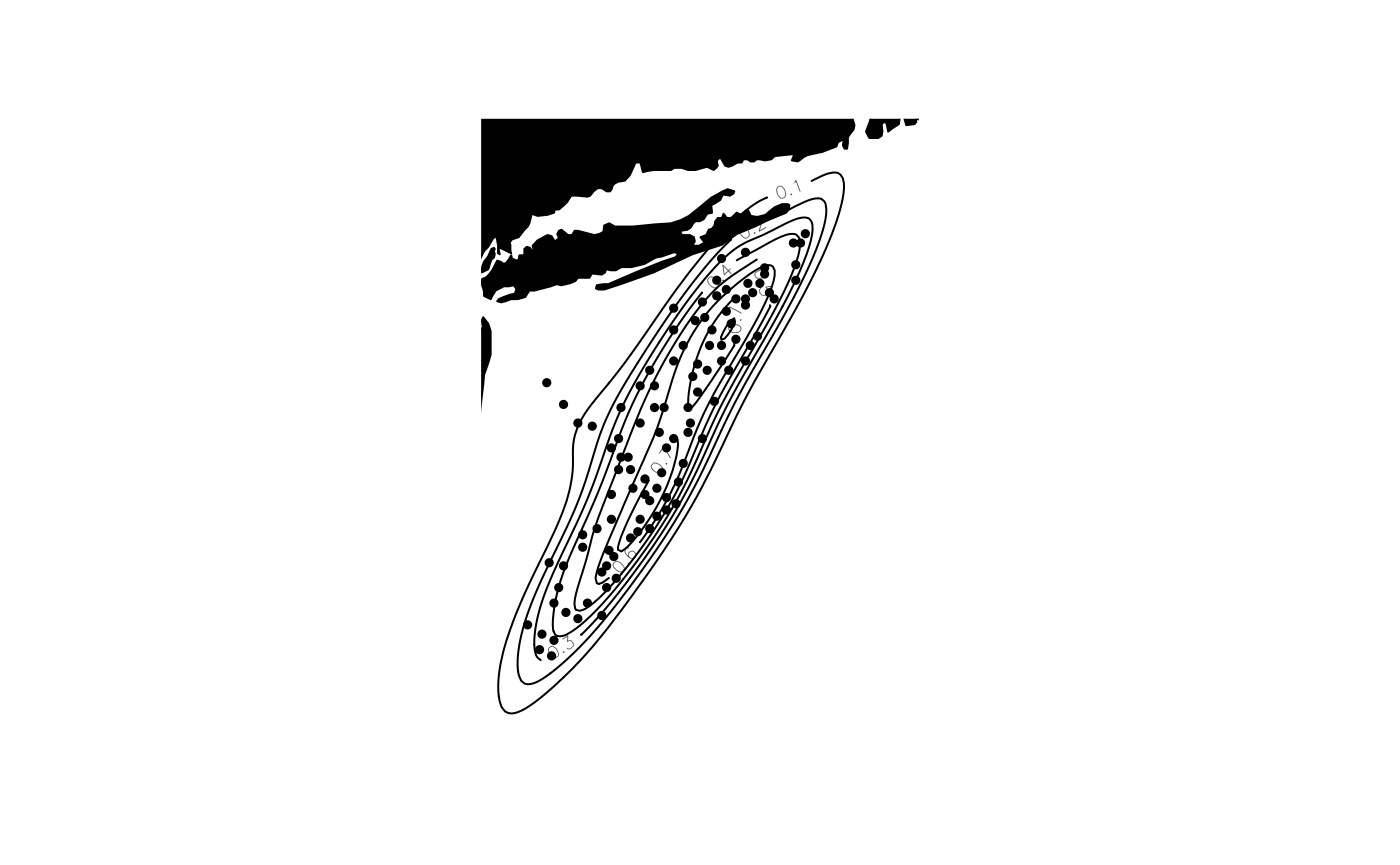
\includegraphics[height=3in]{2b_plot.png}
		\caption{Contour plot}
		\label{fig:contour}
	\end{figure}

\end{enumerate}

\hfill $\blacksquare$


\clearpage
\item

\begin{enumerate}

\item We have the intensity function,
\begin{align*}
	\lambda(t \mid \mathcal{H}_t) &= \mu + \sum_{t_i < t} \frac{k}{(c + t - t_i)^p},
\end{align*}
with $\mu = 1, p = 2, c = 1$, and $k = 0.5$. I will suppress $\mathcal{H}_t$ from the notation for brevity. Thus, we have
\begin{align*}
	\lambda(t) &= 1 + \frac{1}{2} \sum_{t_i < t} \frac{1}{(1 + t - t_i)^2} \\
	&= 1 + \alpha \sum_{t_i < t} \phi(t - t_i).
\end{align*}
Denoting $\psi(s) = \alpha \phi(s)$, where $\phi$ is a density, we can find $\alpha$,
\begin{align*}
	\alpha &= \int_0^{\infty} \psi(s) ds \\
	&= \frac{1}{2} \int_0^{\infty} \frac{1}{(1 + s)^2} ds \\
	&= \frac{1}{2} < 1.
\end{align*}
Therefore, the process is stationary. In particular, note that we have some sufficient and necessary conditions for stationarity: (i) $k < 1$, (ii) $c > 0$, and (ii) $p > 1$. Sufficiency is straightforward. To see necessity, observe that whenever $c \leq 0$, the integrand is not well-defined at $s = -c$. Further, the integral is infinite whenever $p \leq 1$.

So for the remainder of the problem we will assume that $c > 0$ and $p > 1$.

\item The general algorithm is similar to what we saw in class:
\begin{enumerate}
\item Simulate immigrants from Poisson($\mu T$)
\item For each immigrant, choose number of children as Poisson($\alpha$)
\item For each child, choose arrival time (from the parent) as PowerLaw($p-1, c$) where $p-1$ is the shape and $c$ are the scale parameters.
\item Repeat steps 2 and 3 until there are no more children born before $T$
\end{enumerate}

\item From Theorem in class, we know the likelihood is
\begin{align*}
	\mathcal{L} &= \prod_{i=1}^n \lambda(t_i) \cdot \exp\left\{ - \int_0^T \lambda(t) dt \right\} \\
	\implies \ell &= \sum_{i=1}^n \log \lambda(t_i)  - \int_0^T \lambda(t) dt \\
	&= \sum_{i=1}^n \log \left( \mu + \sum_{j=1}^{i-1} \frac{k}{(c + t_i - t_j)^p} \right)  - \int_0^T \lambda(t) dt
\end{align*}
The first term cannot be simplified further. The second term can be computed as
\begin{align*}
	\int_0^T \lambda(t) dt &= \mu T + k \int_0^T \sum_{t_i < t} \frac{1}{(c + t - t_i)^p} dt \\
	&= \mu T + k \sum_{i=1}^{n-1} \int_{t_i}^{t_{i+1}} \sum_{t_j < t} \frac{1}{(c + t - t_j)^p} dt + k \int_{t_n}^{T} \sum_{t_j < t} \frac{1}{(c + t - t_j)^p} dt,
\end{align*}
where we just split the integral into several parts. Now let us look at the second term,
\begin{align*}
	\sum_{i=1}^{n-1} \int_{t_i}^{t_{i+1}} \sum_{t_j < t} \frac{1}{(c + t - t_j)^p} dt &= \sum_{i=1}^{n-1} \sum_{j = 1}^i \int_{t_i}^{t_{i+1}}  \frac{1}{(c + t - t_j)^p} dt \\
	&= \frac{1}{1-p} \sum_{i=1}^{n-1} \sum_{j = 1}^i \left\{ (c + t_{i+1} - t_j)^{1-p} - (c + t_i - t_j)^{1-p} \right\} \\
	&= \frac{1}{1-p} \sum_{i=1}^{n-1} (c + t_n - t_i)^{1-p} - c^{1-p}
\end{align*}
where in the last step, we just expanded out the inner telescoping sum. For the third term,
\begin{align*}
	\int_{t_n}^{T} \sum_{t_j < t} \frac{1}{(c + t - t_j)^p} dt &= \sum_{j=1}^n \int_{t_n}^T \frac{1}{(c + t - t_j)^p} dt \\
	&= \frac{1}{1-p} \sum_{i=1}^n \left\{ (c + T - t_i)^{1-p} - (c + t_n - t_i)^{1-p} \right\}
\end{align*}
Putting it all together, things cancel out as
\begin{align*}
	\int_0^T \lambda(t) dt&= \mu T  + \frac{k}{1 - p} \sum_{i=1}^n \left\{ (c + T - t_i)^{1-p} - c^{1-p} \right\} \\
	\ell &= \sum_{i=1}^n \log \left( \mu + \sum_{j=1}^{i-1} \frac{k}{(c + t_i - t_j)^p} \right) - \mu T  - \frac{k}{1 - p} \sum_{i=1}^n \left\{ (c + T - t_i)^{1-p} - c^{1-p} \right\}
\end{align*}
Compare this with the likelihood obtained for the exponential decay (which is also a part of HW 3). The structure of this equation should be similar. Now, we can feed this into a numerical optimizer.

Although we calculate this by hand and optimize it ourselves for this lab, there are R implementations that do this for us. One such package is \texttt{hawkesbow}. However, as there is no closed-form solution, different implementations may give different results because they rely on different optimization techniques. So try fitting the model with a few different packages. If they all agree, then you have more reason to believe them. If they are all wildly different, something wonky is going on.

\end{enumerate}

\hfill $\blacksquare$


\end{enumerate}





\end{document}


 